\documentclass{standalone}
\usepackage{tikz}
\usetikzlibrary{calc}

\begin{document}

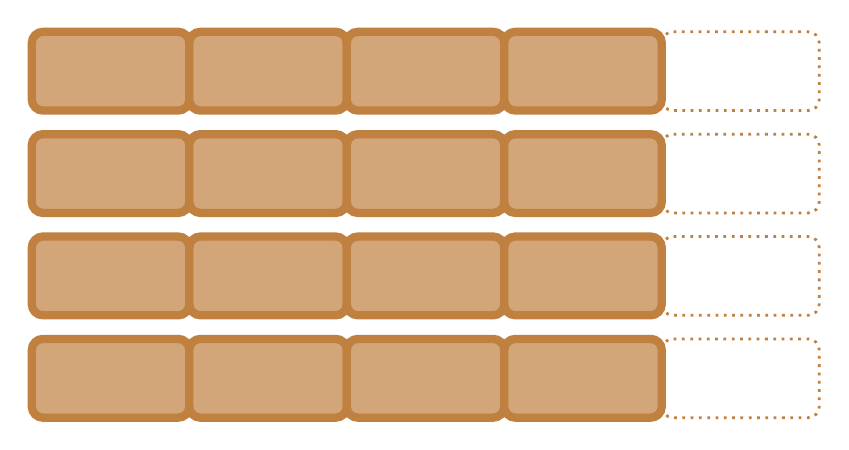
\begin{tikzpicture}[line width=3pt,rounded corners]

\begin{scope}
\fill[draw=brown,fill=brown!70] 								(0,0) rectangle   (2,1);
\fill[draw=brown,fill=brown!70,xshift=2cm] 					   (0,0) rectangle   (2,1);
\fill[draw=brown,fill=brown!70,xshift=4cm] 					   (0,0) rectangle   (2,1);
\fill[draw=brown,fill=brown!70,xshift=6cm] 					   (0,0) rectangle   (2,1);
\draw[draw=brown,xshift=8cm,line width=1pt,draw=brown, dotted] (0,0) rectangle (2,1);
\end{scope}

\begin{scope}[yshift=1.3cm]
\fill[draw=brown,fill=brown!70] (0,0) rectangle   (2,1);
\fill[draw=brown,fill=brown!70,xshift=2cm] (0,0) rectangle   (2,1);
\fill[draw=brown,fill=brown!70,xshift=4cm] (0,0) rectangle   (2,1);
\fill[draw=brown,fill=brown!70,xshift=6cm] (0,0) rectangle   (2,1);
\draw[draw=brown,xshift=8cm,line width=1pt,draw=brown, dotted] (0,0) rectangle (2,1);
\end{scope}

\begin{scope}[yshift=1.3cm*2]
\fill[draw=brown,fill=brown!70] (0,0) rectangle   (2,1);
\fill[draw=brown,fill=brown!70,xshift=2cm] (0,0) rectangle   (2,1);
\fill[draw=brown,fill=brown!70,xshift=4cm] (0,0) rectangle   (2,1);
\fill[draw=brown,fill=brown!70,xshift=6cm] (0,0) rectangle   (2,1);
\draw[draw=brown,xshift=8cm,line width=1pt,draw=brown, dotted] (0,0) rectangle (2,1);
\end{scope}

\begin{scope}[yshift=1.3cm*3]
\fill[draw=brown,fill=brown!70] (0,0) rectangle   (2,1);
\fill[draw=brown,fill=brown!70,xshift=2cm] (0,0) rectangle   (2,1);
\fill[draw=brown,fill=brown!70,xshift=4cm] (0,0) rectangle   (2,1);
\fill[draw=brown,fill=brown!70,xshift=6cm] (0,0) rectangle   (2,1);
\draw[draw=brown,xshift=8cm,line width=1pt,draw=brown, dotted] (0,0) rectangle (2,1);
\end{scope}



\end{tikzpicture}

\end{document}	